% Copyright (C) 2013 - Michael Baudin
%
% This file must be used under the terms of the 
% Creative Commons Attribution-ShareAlike 3.0 Unported License :
% http://creativecommons.org/licenses/by-sa/3.0/

    \chapter{Nets}

%%%%%%%%%%%%%%%%%%%%%%%%%%%%%%%%%%%%%%%%%%%%%%%%%%%%%%%%%%%

\section{Definitions}

The following definition introduces the elementary intervals in one dimensions, 
which are particular intervals in $[0,1)$.

\label{sec-tmsnets-definitions}
\begin{definition}
(\emph{Elementary interval in one dimension.})
Let b be the base, with $b\geq 2$. 
An elementary interval in base b is an interval $[a/b^d,(a+1)/b^d)$
with integers a and d such that $d\geq 0$ and $0\leq a < b^d$.
\end{definition}

Notice that the elementary interval are closed on the left and 
open on the right.

The following definition introduces the multi-dimensional intervals. 

\begin{definition}
(\emph{Multi-dimensional interval.})
The set P is an interval of $[0,1)^s$
if:
$$
P = \prod_{j=1}^s [\alpha_j,\beta_j), 0\leq \alpha_j\leq \beta_j\leq 1,
$$  
for j=1,2,...,s, where $\alpha_j,\beta_j\in[0,1)$ and 
$\alpha_j\leq \beta_j$.
\end{definition}

With low discrepancy sequences, we are interested in specific multi-dimensional intervals, associated 
with a given base $b$.

\begin{definition}
(\emph{Elementary interval in base b in s dimensions.})
Let b be the base, with $b\geq 2$.
An elementary interval in base b of the hypercube $[0,1]^s$ is an interval
$$
\Pi_{i=1}^s [a_i/b^{d_i},(a_i+1)/b^{d_i})
$$
with integers $a_i$ and $d_i$ such that $d_i\geq 0$ and $0\leq a_i < b^{d_i}$,
for $i=1,2,...,s$.
\end{definition}

\begin{corollary}
(\emph{Volume of an elementary interval in base b.})
The volume of an elementary interval in base b in s dimensions is
$$
\frac{1}{b^{d_1+d_2+...+d_s}}.
$$    
\end{corollary}

The following script computes all 
two dimensional elementary intervals in base 2 with area $1/2^3=1/8$, 
and creates the figure \ref{fig-eleminter-v8}.

\lstset{language=scilabscript}
\begin{lstlisting}
scf();
lowdisc_plotbmbox(2,3)
   \end{lstlisting}
	
\begin{figure}[htbp]
\begin{center}
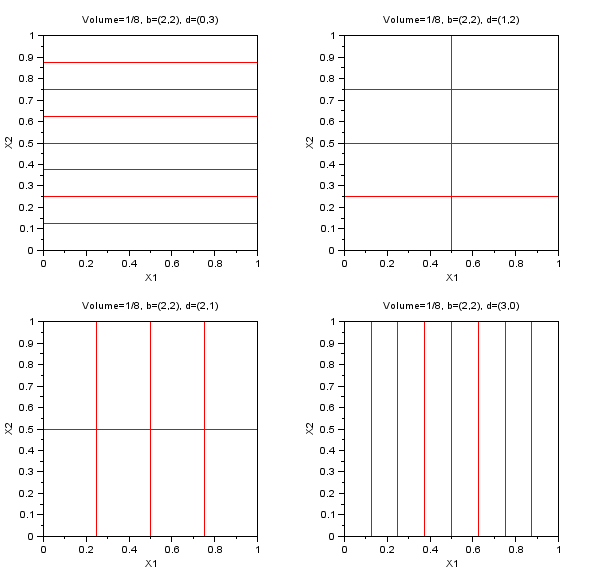
\includegraphics[width=15cm]{figures/eleminter-v8.png}
\end{center}
\caption{Elementary intervals in base 2 with volume 1/8.}
\label{fig-eleminter-v8}
\end{figure}
    
\begin{definition}
(\emph{(t,m,s)-net in base b.})
      Let $b\geq 2$, $s\geq 1$ and $0\leq t\leq m$ be integers.
      Then a point set with $b^m$ points in $[0,1)^s$ is a (t,m,s)-net
      in base b if every elementary interval in base b
      with volume $1/b^{m-t}$ contains exactly $b^t$ points.
\end{definition}

The previous definition is consistent with the fact that the volume 
of the elementary interval is equal to $b^t/b^m$, i.e.
the fraction of points in the elementary interval. 

A smaller base $b$ should be favored because it requires $b^m$ points 
for the property to show up. 
Also, when t decreases, the volume of the associated elementary intervals 
decreases, i.e. even small elementary intervals contain the right number of 
points. 
In other words, a smaller t parameter provides a greater uniformity.

At best, we have $t=0$, for which a point set of $b^m$ points is 
associated with elementary intervals with volume $1/b^m$, 
with one point by elementary interval.

\begin{corollary}
(\emph{(0,m,s)-net in base b.})
      Let $b\geq 2$, $s\geq 1$ be integers.
      Then a point set with $b^m$ points in $[0,1)^s$ is a (0,m,s)-net
      in base b if every elementary interval in base b
      with volume $1/b^m$ contains exactly one point.
\end{corollary}
    

\begin{definition}
(\emph{(t,s)-sequence in base b.})
      Let $b\geq 2$, $s\geq 1$ and $t\geq 0$ be integers.
      Then the infinite sequence $x_0$, $x_1$, ... of points in $[0,1)^s$
      is a (t,s) sequence in base b if,
      for all $k\geq 0$ and $m\geq t$, the point set
$$
x_{kb^m},x_{kb^m+1},...,x_{(k+1)b^m-1},
$$  
      which has $b^m$ points, is a (t,m,s)-net in base $b$.
\end{definition}
    
%%%%%%%%%%%%%%%%%%%%%%%%%%%%%%%%%%%%%%%%%%%%%%%%%%%%%%%%%%%

\section{Theorems}

In this section, we present the main properties of low discrepancy 
sequences in terms of (t,m,s)-nets.

\begin{itemize}

\item Van der Corput in base b are (0,1)-nets in base b.
        
\item Halton sequences are not (t,s)-sequences: the base b is not
          the same for all dimensions. 
          However, a generalized (t,s)-sequence could be defined, 
          with an extended definition taking into account for different 
          bases. 
        
\item Sobol sequence is a (t,s)-sequence in base 2 with t=O(slog(s)).
          Sobol sequence use the same base b=2 for all dimensions.
        
\item The Faure sequences are (0,s)-sequences in base b.
          Therefore, the Faure sequences are (0,m,s)-nets in
          base b, for any $m\geq 0$.
          Therefore, Faure sequences achieve the lowest possible
          value of t, but with increasing b (the smallest prime larger than s).
        
\item Niederreiter sequences are (t,s)-sequences defined for any base b,
          where b is a power of a prime.
\end{itemize}

    
The table \ref{fig-tparameter-sobolnied} presents the quality parameters $t$ of two (t,s)-sequences : 
the Sobol sequence, and the Niederreiter (base 2) sequence.

\begin{figure}
\begin{center}
\begin{tabular}{l|ccccccccccccc}
      s                  & 1 & 2 & 3 & 4 & 5 & 6 &  7 &  8 &  9 & 10 & 11 & 12 & 13 \\
	  \hline
      Niederreiter (b=2) & 0 & 0 & 1 & 3 & 5 & 8 & 11 & 14 & 18 & 22 & 26 & 30 & 34 \\
      Sobol              & 0 & 0 & 1 & 3 & 5 & 8 & 11 & 15 & 19 & 23 & 27 & 31 & 35 \\
\end{tabular}

\begin{tabular}{l|ccccccc}
      s                  & 14 & 15 & 16 & 17 & 18 & 19 & 20 \\
	  \hline
      Niederreiter (b=2) & 38 & 43 & 48 & 53 & 58 & 63 & 68 \\
      Sobol              & 40 & 45 & 50 & 55 & 60 & 65 & 71 \\
\end{tabular}

\begin{tabular}{l|cccccccccc}
      s                  & 21 & 22 & 23 & 24 &  25 &  26 &  27 &  28 &  29 &  30 \\
	  \hline
      Niederreiter (b=2) & 73 & 78 & 83 & 89 &  95 & 101 & 107 & 113 & 119 & 125 \\
      Sobol              & 77 & 83 & 89 & 95 & 101 & 107 & 113 & 119 & 125 & 131 \\
\end{tabular}

\begin{tabular}{l|cccccccccc}
      s     &  31 &  32 &  33 &  34 &  35 &  36 &  37 &  38 &  39 &  40 \\
	  \hline
      Sobol & 137 & 143 & 149 & 155 & 161 & 167 & 173 & 180 & 187 & 194 \\
\end{tabular}
\end{center}
\caption{The quality parameter $t$ for the Sobol and Niederreiter sequences.}
\label{fig-tparameter-sobolnied}
\end{figure}

%%%%%%%%%%%%%%%%%%%%%%%%%%%%%%%%%%%%%%%%%%%%%%%%%%%%%%%%%%%

\section{Discrepancy}
    
\begin{definition}
(\emph{Star intervals.})
The $I^\star$ set is the set of origin-anchored
      intervals in $[0,1]^s$:
$$
        I^\star = \left\{P=\prod_{j=1}^s [0,\beta_j), 0\leq \beta_j\leq 1\right\}.
$$    
\end{definition}
    
\begin{definition}
(\emph{Number of points and volume of an interval.})
      Let $x$ be a sequence of more than $n$ points in $[0,1)^s$.
      Then $x(n)$ represents the set of the first $n$ points of the sequence $x$.
      Let $P$ be an interval of $[0,1)^s$.
      Therefore, the number $A(P,x(n))$ is the number of points 
	  from $x(n)$ in the interval P.
      Moreover, let $\lambda(P)$ be the volume of P:
$$
        \lambda(P) = \lambda(P)\prod_{j=1}^s (\beta_j-\alpha_j)
$$    
\end{definition}

\begin{definition}
(\emph{Star discrepancy.})
      Let $x$ be a sequence of more than n points in $[0,1)^s$.
      The star discrepancy $D^\star(x)$ measures the lack of uniformity of the
      first $n$ points:    
$$
        D^\star_n(x)=\sup_{P\in I^\star} \left| \frac{1}{n}A(P,x(n)) - \lambda(P) \right|.
$$    
\end{definition}

%%%%%%%%%%%%%%%%%%%%%%%%%%%%%%%%%%%%%%%%%%%%%%%%%%%%%%%%%%%

\section{Estimate of the mean by a low discrepancy sequence}

    
\begin{theorem}
(\emph{Koksma-Hlawka.})
      Let f from $[0,1)^s$ to $\RR$ be a function where
      $V(f)$, the variation in the sense of Hardy and Krause, is bounded, therefore,
      for any sequence of n points $x(n)$, we have
$$
        \left|\frac{1}{n} \sum_{i=1}^n f\left(x^{(i)}\right) - \int_{[0,1]^s} f(x)dx \right|
        \leq V(f) D^\star_n(x).
$$    
\end{theorem}

\begin{theorem}
(\emph{Niederreiter.})
      For any (t,s)-sequence in base b, we have
$$
        D^\star_n(x) \leq C(b,s,t) n^{-1} (\log n)^s + O\left(n^{-1} (\log n)^{s-1}\right)
$$
\end{theorem}

In other words, any (t,s)-sequence is a low discrepancy sequence.

In the previous inequality, the dominating term, when $n$ is large, is $1/n$.
However, for moderate n, the factor $\log(n)^s$ must be taken into account.
Indeed, we the function $\log(n)^s/n$ increases for n lower than $\exp(s)$.
In other words, for increasing values of s, the number of points n
required to get into the asymptotic discrepancy rate is larger and larger.


\begin{itemize}
        
\item Sobol sequence : $C(b,s,t)$ grows to infinity, when s increases.
        
\item Faure sequences : $C(b,s,t)$ grows to zero, when s increases.
        
\item Niederreiter sequences : $C(b,s,t)$ grows to zero, when s increases.
\end{itemize}



The table \ref{fig-Cbst-halsofanied} presents the constant $C(b,s,t)$ for several
sequences.

\begin{figure}
\begin{center}
\begin{tabular}{l|ccccccccc}
s       & 2     & 3     & 4     & 5     & 6     & 7      & 8      & 9        & 10       \\
\hline
Halton  & 0.65  & 0.81  & 1.25  & 2.62  & 6.13  & 17.3   & 52.9   & 185.5    & 771.5    \\
Sobol   & 0.26  & 0.25  & 0.541 & 0.833 & 1.6   & 2.6    & 7.6    & 19.6     & 45.0     \\
Faure   & 0.26  & 0.13  & 0.099 & 0.025 & 0.019 & 0.0041 & 0.0089 & $2.1\times 10^{-3}$ & $4.2\times 10^{-4}$ \\
Nieder. & 0.26  & 0.13  & 0.086 & 0.025 & 0.019 & 0.0041 & 0.0030 & $6.1\times 10^{-4}$ & $4.2\times 10^{-4}$ \\
\end{tabular}
\end{center}
\caption{The constant $C(b,s,t)$ for various low discrepancy sequences.}
\label{fig-Cbst-halsofanied}
\end{figure}

%%%%%%%%%%%%%%%%%%%%%%%%%%%%%%%%%%%%%%%%%%%%%%%%%%%%%%%%%%%

\section{Halton sequence}

In this section, we show how the Halton sequence fill elementary intervals 
for which the $i$-th side has length equal to a power of $1/b_i$, where 
$b_i$ is the prime number associated with the $i$-th coordinate. 

In the following script, we consider the first $2^2\times 3=12$ points of the 
Halton sequence in two dimensions. 
Then we consider elementary intervals of area $1/12$, where 
the sides of the intervals have length equal to $1/2^2$ and $1/3$. 

\lstset{language=scilabscript}
\begin{lstlisting}
// Get the points 0,1,...,11 (insert zero)
u=lowdisc_ldgen ( 11 , 2 , "halton" );
u = [0,0;u];
//
scf();
subplot(1,2,1);
plot(u(:,1),u(:,2),"bo")
lowdisc_plotelembox([2 3],[2 1])
xtitle("Halton, Volume=1/12, 12 Points");
h = gca();
h.isoview="off";
//
subplot(1,2,2);
plot(u(:,1),u(:,2),"bo")
lowdisc_plotelembox([2 3],[1 1])
xtitle("Halton, Volume=1/6, 12 Points");
h = gca();
h.isoview="off";
   \end{lstlisting}
    
The previous script produces the figure \ref{fig-halton-n12}.

\begin{figure}[htbp]
\begin{center}
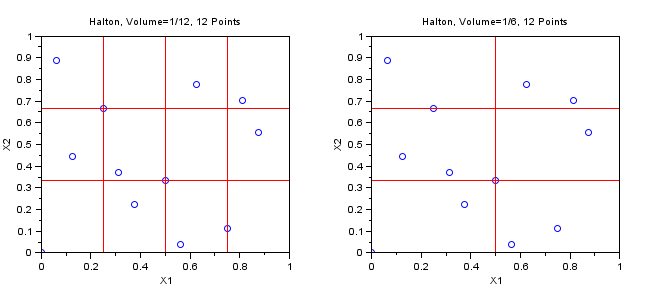
\includegraphics[width=15cm]{figures/halton-n12.png}
\end{center}
\caption{The Halton sequence : 12 points with elementary intervals of volume 1/6.}
\label{fig-halton-n12}
\end{figure}

We see that there are exactly $6/12=2$ points in each interval. 

%%%%%%%%%%%%%%%%%%%%%%%%%%%%%%%%%%%%%%%%%%%%%%%%%%%%%%%%%%%

\section{Faure sequence}
\label{sec-tmsnetfaure}

In dimension s=2, the Faure sequence uses the base 2. 
Moreover, the Faure sequence is a (0,2)-sequence in base 2 
(i.e. the quality parameter t is zero). 
We choose m=4, and check that Faure is a (0,4,2)-net in base 2. 
Hence, we have to consider $b^m=2^4=16$ points and check that 
there are $b^t=1$ points for any elementary interval of area 
$1/b^m=1/16$.

In the following script, we consider $2^4=16$ 
Faure points and plot elementary intervals with area $1/2^4=1/16$. 
We want to check that there is 1 point by elementary interval.    

\lstset{language=scilabscript}
\begin{lstlisting}
u=lowdisc_ldgen ( 2^4-1 , 2 , "faure" );
u = [0,0;u];
scf();
lowdisc_plotbmbox(2,4,u);
\end{lstlisting}

The previous script produces the figure \ref{fig-faure-n16-v16}.

\begin{figure}[htbp]
\begin{center}
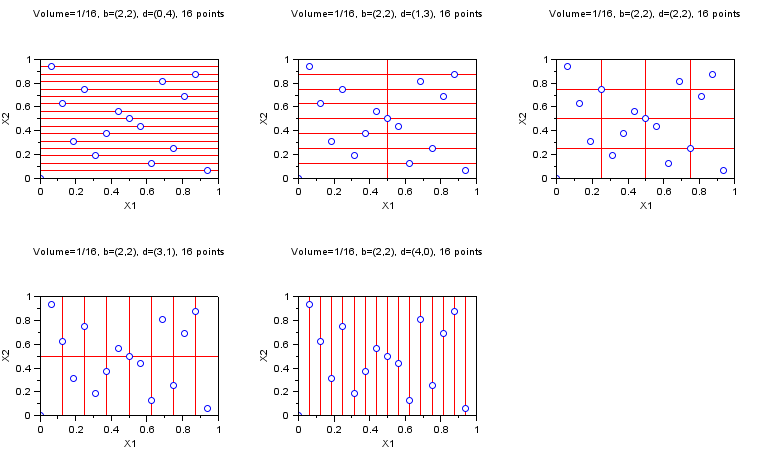
\includegraphics[width=15cm]{figures/faure-n16-v16.png}
\end{center}
\caption{The Faure sequence : 16 points with elementary intervals of volume 1/16.}
\label{fig-faure-n16-v16}
\end{figure}
    

    
In the following script, we consider $2^4=16$ Faure points in two dimensions 
and plot elementary intervals with area $1/2^3=1/8$:
there are 2 points by box.   

\lstset{language=scilabscript}
\begin{lstlisting}
u=lowdisc_ldgen ( 2^4-1 , 2 , "faure" );
u = [0,0;u];
scf();
lowdisc_plotbmbox(2,3,u);
   \end{lstlisting}

   The previous script produces the figure \ref{fig-faure-n16-v8}.

\begin{figure}[htbp]
\begin{center}
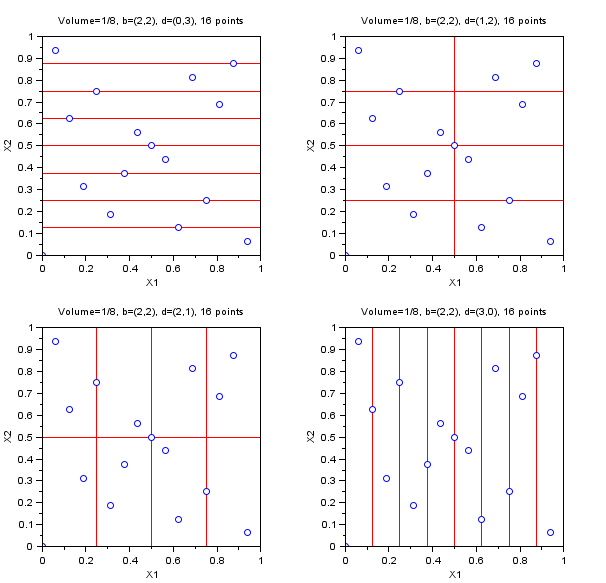
\includegraphics[width=15cm]{figures/faure-n16-v8.png}
\end{center}
\caption{The Faure sequence : 16 points with elementary intervals of volume 1/8.}
\label{fig-faure-n16-v8}
\end{figure}
    

    
In the following script, we consider 16 Faure points in two dimensions 
and plot elementary intervals with volume $1/8$.

\lstset{language=scilabscript}
\begin{lstlisting}
// Get the points 0,1,...,15 (insert zero)
u=lowdisc_ldgen ( 2^4-1 , 2 , "faure" );
u = [0,0;u];
scf();
//
subplot(2,2,1);
plot(u(1:8,1),u(1:8,2),"bo")
plot(u(9:16,1),u(9:16,2),"g*")
legend(["Points 1-8","Points 9-16"]);
lowdisc_plotelembox(2,[3 0]);
xtitle("Faure, Volume=1/8, 16 Points");
h = gca();
h.isoview="off";
//
subplot(2,2,2);
plot(u(1:8,1),u(1:8,2),"bo")
plot(u(9:16,1),u(9:16,2),"g*")
legend(["Points 1-8","Points 9-16"]);
lowdisc_plotelembox(2,[2 1]);
xtitle("Faure, Volume=1/8, 16 Points");
h = gca();
h.isoview="off";
//
subplot(2,2,3);
plot(u(1:8,1),u(1:8,2),"bo")
plot(u(9:16,1),u(9:16,2),"g*")
legend(["Points 1-8","Points 9-16"]);
lowdisc_plotelembox(2,[0 3]);
xtitle("Faure, Volume=1/8, 16 Points");
h = gca();
h.isoview="off";
//
subplot(2,2,4);
plot(u(1:8,1),u(1:8,2),"bo")
plot(u(9:16,1),u(9:16,2),"g*")
legend(["Points 1-8","Points 9-16"]);
lowdisc_plotelembox(2,[1 2]);
xtitle("Faure, Volume=1/8, 16 Points");
h = gca();
h.isoview="off";
   \end{lstlisting}

   The previous script produces the figure \ref{fig-faure-n16-v8-bis}.
We check that there are two points by interval.
Moreover, the first 8 points fill all intervals (1 point by interval),
while the points from 9 to 16 again fill the intervals. 

\begin{figure}[htbp]
\begin{center}
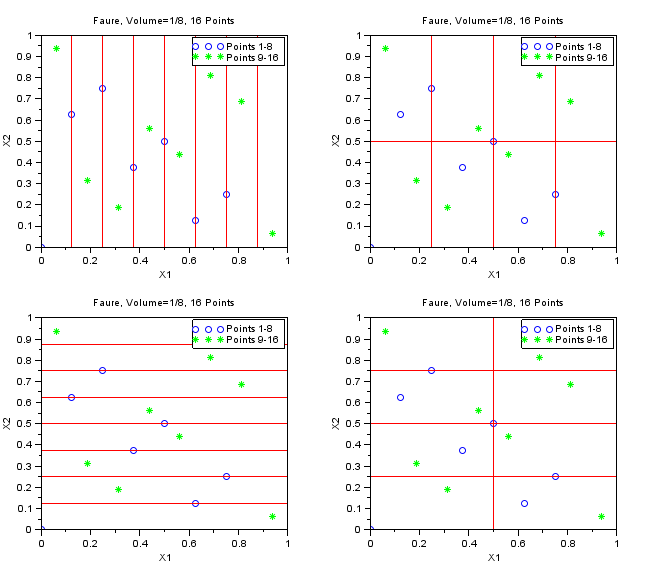
\includegraphics[width=15cm]{figures/faure-n16-v8-bis.png}
\end{center}
\caption{The Faure sequence : 16 points with elementary intervals of volume 1/8.}
\label{fig-faure-n16-v8-bis}
\end{figure}
    
    
%%%%%%%%%%%%%%%%%%%%%%%%%%%%%%%%%%%%%%%%%%%%%%%%%%%%%%%%%%%


\section{Niederreiter base 2 sequence}

In the following script, we consider $2^5=32$ Niederreiter (base 2) points 
in two dimensions and plot elementary intervals with area $2^4$:
there are 2 points by elementary interval. 
Indeed, Niederreiter is a (0,5,2)-net in base 2
    
\lstset{language=scilabscript}
\begin{lstlisting}
u=lowdisc_ldgen ( 2^5-1 , 2 , "niederreiter" );
u = [0,0;u];
scf();
lowdisc_plotbmbox(2,4,u);
    \end{lstlisting}
    
The previous script produces the figure \ref{fig-nieder-n32-v16}.

\begin{figure}[htbp]
\begin{center}
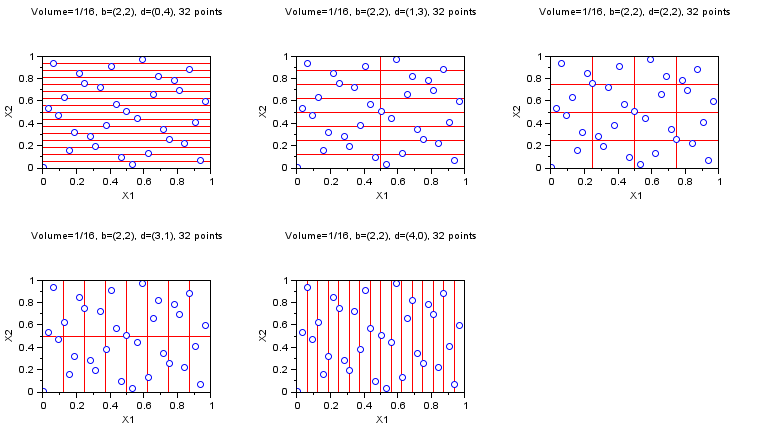
\includegraphics[width=15cm]{figures/nieder-n32-v16.png}
\end{center}
\caption{The Niederreiter sequence : 32 points in 2 dimensions, with 
elementary intervals of area $1/16$.}
\label{fig-nieder-n32-v16}
\end{figure}
    
    
In the following script, we consider $2^5=32$ Niederreiter (base 2) points in 
two dimensions and plot elementary intervals with area $2^3=8$:
there are 4 points by elementary interval.
Indeed, Niederreiter is a (0,5,2)-net in base 2
    
\lstset{language=scilabscript}
\begin{lstlisting}
u=lowdisc_ldgen ( 2^5-1 , 2 , "niederreiter" );
u = [0,0;u];
scf();
lowdisc_plotbmbox(2,3,u);
\end{lstlisting}

The previous script produces the figure \ref{fig-nieder-n32-v8}.

\begin{figure}[htbp]
\begin{center}
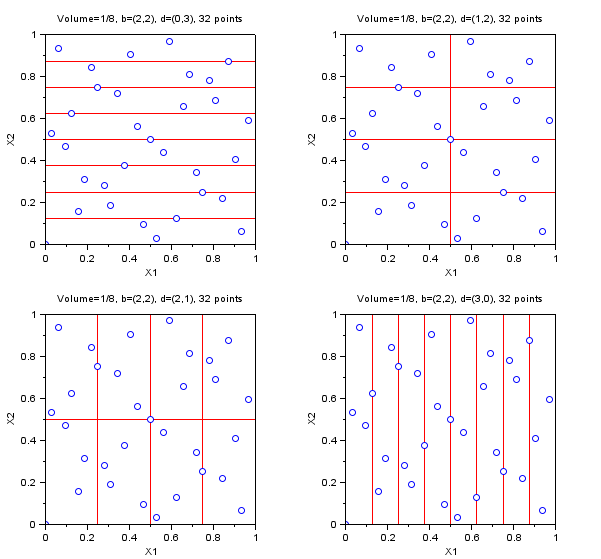
\includegraphics[width=15cm]{figures/nieder-n32-v8.png}
\end{center}
\caption{The Niederreiter sequence : 32 points in 2 dimensions, with 
elementary intervals of area $1/8$.}
\label{fig-nieder-n32-v8}
\end{figure}

  
%%%%%%%%%%%%%%%%%%%%%%%%%%%%%%%%%%%%%%%%%%%%%%%%%%%%%%%%%%%


\section{Sobol sequence}

    
Sobol is a (0,4,2)-net in base 2. 
To check this, we consider $2^4=16$ Sobol points in two dimensions, 
and plot elementary intervals with area $1/16$: 
there is 1 point by elementary interval.
To plot the elementary intervals, we use $2^2$ subdivisions for $X_1$,
and $2^2$ subdivisions for $X_2$.
    
\lstset{language=scilabscript}
\begin{lstlisting}
u=lowdisc_ldgen ( 2^4-1 , 2 , "sobol" , %t );
u = [0,0;u];
h = scf();
lowdisc_plotbmbox(2,4,u);
    \end{lstlisting}

    
The previous script produces the figure \ref{fig-sobol-n16-v16}.

\begin{figure}[htbp]
\begin{center}
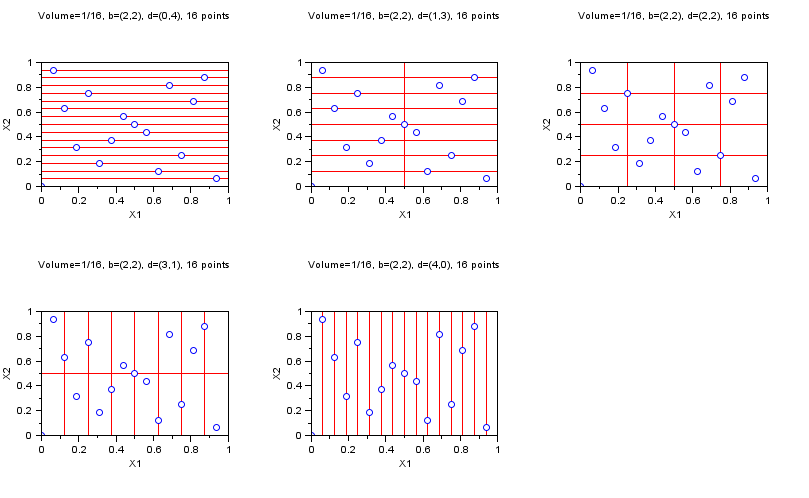
\includegraphics[width=15cm]{figures/sobol-n16-v16.png}
\end{center}
\caption{The Sobol sequence : 16 points in 2 dimensions, with 
elementary intervals of area $1/16$.}
\label{fig-sobol-n16-v16}
\end{figure}
    
Sobol is a (0,5,2)-net in base 2.
In order to check this, we consider $2^6=64$ Sobol points in two dimensions 
and plot elementary intervals with area $1/32$:
there are two points by elementary interval. 
The elementary intervals tse $2^3$ subdivisions for $X_1$ 
and $2^2$ subdivisions for $X_2$.
    
\lstset{language=scilabscript}
\begin{lstlisting}
u=lowdisc_ldgen ( 2^6-1 , 2 , "sobol" );
u = [0,0;u];
h = scf();
plot(u(1:2^5,1),u(1:2^5,2),"bo")
plot(u(2^5+1:2^6,1),u(2^5+1:2^6,2),"g*")
legend(["Points 1-32","Points 33-64"]);
lowdisc_plotelembox(2,[3 2]);
xtitle("Sobol, Volume=1/32, 64 Points");
    \end{lstlisting}

The previous script produces the figure \ref{fig-sobol-n64-v32}.

\begin{figure}[htbp]
\begin{center}
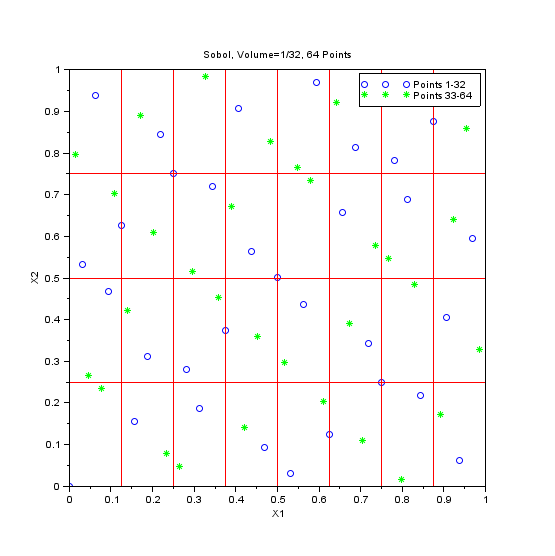
\includegraphics[width=15cm]{figures/sobol-n64-v32.png}
\end{center}
\caption{The Sobol sequence : 64 points in 2 dimensions, with 
elementary intervals of area $1/32$.}
\label{fig-sobol-n64-v32}
\end{figure}

%%%%%%%%%%%%%%%%%%%%%%%%%%%%%%%%%%%%%%%%%%%%%%%%%%%%%%%%%%%


\section{Leaped sequences and (t,m,s)-nets}
    
A common practice is to use a leaped sequence to 
improve the correlations in high dimensions. 
However, we may notice that a leaped sequence 
may lead to a set which is not a (t,m,s)-net anymore.

In \cite{Kocis1997} (p. 274), Kocis and Whiten suggest to use leaped sequences, as 
presented in the figure \ref{fig-leapprinciple}. 
In such a Halton leaped sequence, we use every (L+1)-th 
vector, subject to the condition that $L+1$ is a prime different 
from all bases. 
Hence, when $L=0$, all elements are considered while when $L=1$, 
only one element every two numbers is used. 

\begin{figure}[htbp]
\begin{center}
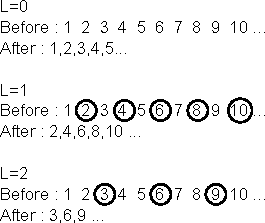
\includegraphics[width=6cm]{figures/leaping-principle}
\end{center}
\caption{Principle of the leap parameter.}
\label{fig-leapprinciple}
\end{figure}

Kocis and Whiten use test functions with the goal of finding 
the leaps which minimizes the integration error. 
They do this experiment with s in the range from 1 to 400, 
a number of points from 10 to $10^5$ and a leap 
parameter in the range from 3 to 3000. 
They find that the best values for $L+1$ are 31, 61, 149, 409, and 1949. 
This suggests to use L+1=409 for dimensions less than 400. 

For example, let's see the first 12 points of a leaped
Halton sequence in two dimensions, and consider elementary intervals with area 
$1/12$. 
    
\lstset{language=scilabscript}
\begin{lstlisting}
u=lowdisc_ldgen ( 11 , 2 , "halton" , %f );
u = [0,0;u];
//
scf();
subplot(1,2,1);
plot(u(:,1),u(:,2),"bo")
lowdisc_plotelembox([2 3],[2 1])
xtitle("Halton, Volume=1/12, 12 Points");
h = gca();
h.isoview="off";
//
subplot(1,2,2);
plot(u(:,1),u(:,2),"bo")
lowdisc_plotelembox([2 3],[1 1])
xtitle("Halton, Volume=1/6, 12 Points");
h = gca();
h.isoview="off";
    \end{lstlisting}

    
The previous script produces the figure \ref{fig-halton-leaped-s2}. 
In this experiment, we use $L+1=5$, i.e. the third prime number. 
This is because the primes $b_1=2$ and $b_2=3$ are used for the 
dimensions 1 and 2. 
Although the unleaped Halton sequence had exactly 1 point
by elementary interval, the leaped Halton sequence is not
as regular : some intervals are empty (the top left on the left
figure), some intervals have more points than expected 
(the bottom left on the left figure).

\begin{figure}[htbp]
\begin{center}
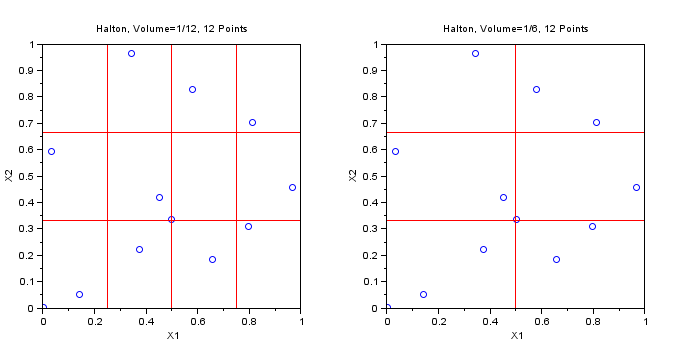
\includegraphics[width=15cm]{figures/halton-leaped-s2.png}
\end{center}
\caption{The leaped Halton sequence : 12 points in 2 dimensions, 
with elementary intervals of area $1/6$.}
\label{fig-halton-leaped-s2}
\end{figure}
    
The same phenomenon may happen with a leaped Faure sequence. 
In the following script, we consider $2^4=16$ points in 2 dimensions, 
with elementary intervals of area $1/16$. 
We use the leap parameter $L=5$.

\lstset{language=scilabscript}
\begin{lstlisting}
lds = lowdisc_new("faure");
lds = lowdisc_configure(lds,"-dimension",2);
lds = lowdisc_configure(lds,"-leap",5);
lds = lowdisc_startup (lds);
[lds,u] = lowdisc_next (lds,2^4-1);
lds = lowdisc_destroy(lds);
u = [0,0;u];
scf();
lowdisc_plotbmbox(2,4,u);
\end{lstlisting}
    
The previous script produces the figure \ref{fig-faure-leaped-s2}.

\begin{figure}[htbp]
\begin{center}
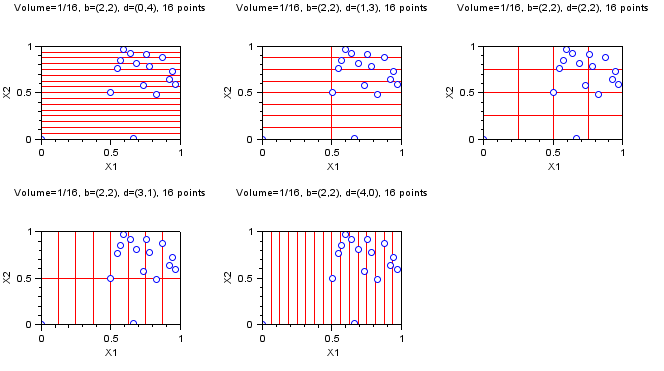
\includegraphics[width=15cm]{figures/faure-leaped-s2.png}
\end{center}
\caption{The leaped Faure sequence : $2^4=16$ points in 2 dimensions, 
with elementary intervals of area $1/16$.}
\label{fig-faure-leaped-s2}
\end{figure}

%%%%%%%%%%%%%%%%%%%%%%%%%%%%%%%%%%%%%%%%%%%%%%%%%%%%%%%%%%%

\section{Notes and references}

Most of the content of the section  \ref{sec-tmsnets-definitions} is 
based on Niederreiter's \cite{Niederreiter1992}. 
This is also partly based on Glasserman's \cite{Glasserman2003}, 
especially section 5.1.4 "Nets and sequences", and Fig. 5.3, page 292.

Some of the $(t,m,s)$-nets plots of the section \ref{sec-tmsnetfaure} can be seen 
in \cite{Seng1997} or in \cite{Thiemard2000} (see Fig 4.7).

The table \ref{fig-Cbst-halsofanied} is the table 4.2 in \cite{Thiemard2000} (Section 4.6 "Les (t,s)-suites 
et les (t,m,s)-reseaux. and Fig 4.7).

The table \ref{fig-tparameter-sobolnied} presents the quality parameters $t$ of two (t,s)-sequences. 
For Sobol sequence, this is the table in section 3.4 of \cite{rBRA88c}, 
extended with personal computations.
For the Niederreiter sequence in base 2, this is the table II in \cite{Niederreiter1988}.
